\chapter{Quasicrystals}
\begin{figure}[h] %[h] para here [b] para bottom [t] para top
\centering
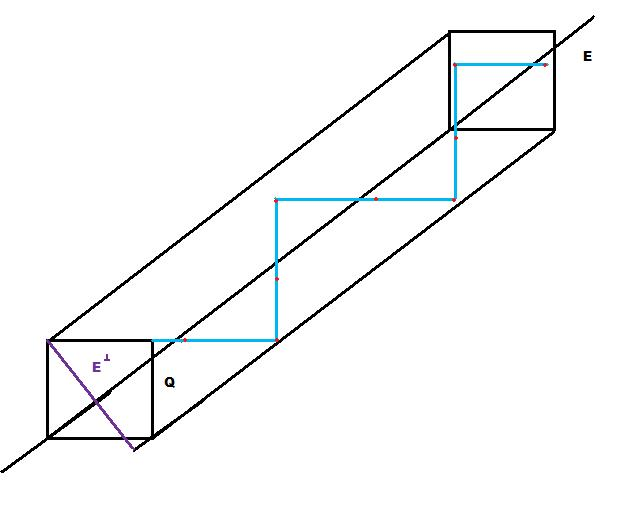
\includegraphics[width=250pt]{./graphics/Quasi.jpg}
%\caption{Ejemplos de cada tipo de juego}
\end{figure}
We pick
$$\textbf{E}=\{\vec{x}\in\RR^2\ |\ x_2=x_1\cdot c,\ c\in\RR\setminus\QQ\}.$$
There are $2$ kind of segments the big ones and the smaller ones the proportion is $c$.\smallskip\\
$\textbf{E}^{\bot}$ is dense $\Rightarrow 2^{\NN}$ is $\infty$ no countable.\smallskip\\
We can generalize this to any parallelepiped and if we are in a lattice the canonical projetion method picks $\Vor(0)$ as $Q$. It is also possible in higher dimensions.\smallskip\\
Given $x\in L$, $\textbf{E}\subset \RR^d$, $Q\subseteq\RR^d$ we have to decide whether $x\in\mathbf{E}+Q$.\smallskip\\
We project $Q$ and $x$ onto $\pi_{\textbf{E}^{\bot}}(\mathbf{E}+Q)$, where $\pi_{\textbf{E}^{\bot}}$ is the projection window, if $x^{'}\in Q^{'}\Leftrightarrow x\in\mathbf{E}+Q$.